\documentclass[handout]{beamer}
%\documentclass{beamer}
\usepackage{tikz}
\def\checkmark{\tikz\fill[scale=0.4](0,.35) -- (.25,0) -- (1,.7) -- (.25,.15) -- cycle;} 
\usepackage{pifont}
\newcommand{\xmark}{\ding{55}}
\usepackage{tikz}
\usepackage{biblatex}
\usetheme{PaloAlto}
\title{The (many) benefits of simulated data}
\author[Ben Lambert]{Ben Lambert\inst{1}\\ \texttt{ben.c.lambert@gmail.com}}

\usepackage{datetime}
\newdate{date}{23}{6}{2021}
\date{\displaydate{date}}
\institute[University of Oxford]{
\inst{1}University of Oxford}
\beamertemplatenavigationsymbolsempty
\setbeamertemplate{sidebar left}{}
\usepackage{caption}
\usepackage{amsmath}
\usepackage{soul,xcolor}
\usepackage{multimedia}
\usepackage{bbm}
\usepackage{animate}
\usepackage{graphics}
\usepackage{graphicx}
\usepackage[makeroom]{cancel}
\usepackage{xcolor,cancel}
\captionsetup{font=footnotesize}
\usepackage[utf8]{inputenc}
\makeatletter
\newcommand\mathcircled[1]{%
  \mathpalette\@mathcircled{#1}%
}
\newcommand\@mathcircled[2]{%
  \tikz[baseline=(math.base)] \node[draw,circle,inner sep=1pt] (math) {$\m@th#1#2$};%
}
\makeatother
\definecolor{beige}{RGB}{238,213,173}

\newcommand\hcancel[2][black]{\setbox0=\hbox{$#2$}%
	\rlap{\raisebox{.45\ht0}{\textcolor{#1}{\rule{\wd0}{1pt}}}}#2} 

\bibliography{Bayes}

\begin{document}

\begin{frame}
\titlepage
\end{frame}

\begin{frame}
	\frametitle{Course plan}
	\begin{itemize}
		\item 9.30am-10.15am: lecture, ``The benefits of simulated data''
		\item 10.45am-1pm: practical
		\item 2pm-2.30pm: lecture, ``Reproducible data analysis''
		\item 2.45pm-5pm: practical
	\end{itemize}
	
\end{frame}

\begin{frame}
	\frametitle{Lecture content}
	
	\begin{itemize}
		\item How to create useful methods (using simulation)
		\item Two key problems with statistical significance testing (explored via simulation in problem sets)
		\item Simulated data for inference and experimental design
	\end{itemize}
	
\end{frame}

\begin{frame}
	\frametitle{Outline}
	\tableofcontents
\end{frame}

\section{How to create useful methods}
\frame{\tableofcontents[currentsection]}

\begin{frame}
	\frametitle{Null hypothesis testing}
	
	Assume we have a null hypothesis $H_0$ for how data are generated. For example, suppose:
	
	\begin{equation}
	X_i \sim \text{normal}(\theta, 1),
	\end{equation}
	
	where $H_0: \theta=0$ versus an alternative hypothesis (say) $H_1: \theta < 0$.
	
\end{frame}

\begin{frame}
	\frametitle{$p$-values}
	
	In statistical hypothesis testing, the $p$-value is the probability of observing something as least as extreme as the observed test statistic, $T(X)$:
	
	\begin{equation}
	p = \mathbb{P}(T(X^{\text{rep}}) \leq T(X)),
	\end{equation}
	
	where if $H_0: \theta=0$,
	
	 \begin{equation}
	 X_i \sim \text{normal}(0, 1).
	 \end{equation}
	 
	 and we could have $X^{\text{rep}} = (X_1, X_2, ..., X_N)$ and
	 
	 \begin{equation}
	 T(X^{\text{rep}}) = \frac{1}{N}\sum_{i=1}^{N} X_i.
	 \end{equation}
	
\end{frame}

\begin{frame}
	\frametitle{Statistical test size}
	
	\begin{itemize}
		\item Reject $H_0$: $p \leq \alpha$,
		\item Do not reject $H_0$: $p > \alpha$.
	\end{itemize}
	
	Here,
	
	\begin{equation}
	\alpha = \mathbb{P}(\text{conclude } H_0 \text{ is false}|H_0 \text{ is true})
	\end{equation}
	
	is known as the size of a statistical test.
	
\end{frame}

\begin{frame}
	\frametitle{Statistical power}
	
	Suppose some alternative hypothesis $H_1: \theta = \theta_1$ is true, then:
	 
	 \begin{equation}
	 \text{power} = \mathbbm{P}(\text{reject } H_0| H_1 \text{ is true})
	 \end{equation}
	 
	 
	 So power relates to a \textbf{specific} alternative hypothesis, $H_1$; a test that's good for one $H_1$ may not be good at many others.
	 
	 \vspace{0.5cm}
	 
	 It's also typically defined relative to a given $\alpha$ value: for example, ``the power to reject the null against specific $H_1$ using a statistical significance of $Y$''.
	 
\end{frame}

\begin{frame}
	\frametitle{Designing methods}
	
	\begin{itemize}
		\item Many of you will create methods for use by others
		\item Important to ensure this is done responsibly so it can be replicated: good software testing and comprehensively documented
		\item As important is to ensure that the methods are \textbf{useful}
	\end{itemize}
	
\end{frame}

\begin{frame}
	\frametitle{How to create and publish useful tests}
	
	Whilst there are many types of method, here we use statistical tests as a case study in ensuring usefulness.
	
	\vspace{0.5cm}
	
	A statistical test is useful if:
	
	\begin{enumerate}
		\item Its $\alpha$ behaves as it should under the distribution(s) defined by the null hypothesis
		\item It is powerful across a range of likely to be encountered $H_1$s
		\item You have determined and communicated the $H_1$s for which it doesn't work
	\end{enumerate}
	
	$\implies$ can use simulation to handle all the above!
	
\end{frame}

\begin{frame}
	\frametitle{1. Checking $\alpha$}
	
	I wrote the following imprecise statement for the null distribution of a single data point:
	
	\begin{equation}
	X_i \sim \text{normal}(0, 1).
	\end{equation}
	
	There are a number of ways this could be true. For example,
	
	\begin{equation}
	X_i \stackrel{i.i.d.}{\sim} \text{normal}(0, 1).
	\end{equation}	
	
	Or (say),
	
	\begin{equation}
	X_i = \rho X_{i-1} + \epsilon_i,
	\end{equation}
	
	where $|\rho|<1$ and $\epsilon_i \stackrel{i.i.d.}{\sim} \text{normal}(0,\sqrt{1-\rho^2})$.
	
	\textbf{Question}: does your $\alpha$ behave as expected under these ranges? Or do you need to be more specific when defining $H_0$.
	
\end{frame}


\begin{frame}
	\frametitle{2. and 3. checking power under a variety of $H_1$s}
	
	Assume null distribution: $X \stackrel{i.i.d.}{\sim} \text{normal}(0, 1)$. There are a variety of alternative hypotheses:
	
	\begin{itemize}
		\item $H_1: X \sim \text{normal}(-1, 1)$
		\item $H_1: X \sim \text{normal}(0, 1.5)$
		\item $H_1: X \stackrel{\text{non } i.i.d.}{\sim} \text{normal}(0, 1)$
		\item $H_1: X\sim \text{Student-t}(...)$
		\item $H_1: X \sim \text{skew-normal}(...)$
		\item $H_1: X \sim \text{multimodal-normal}(...)$
	\end{itemize}
	
	Note, if all the above were relevant, you should communicate power results across all of these: good and bad.
	
\end{frame}

\section{Two key problems with statistical significance testing}
\frame{\tableofcontents[currentsection]}

\begin{frame}
	\frametitle{Statistical significance is not practical significance}
	
	Suppose two treatments aimed at increasing personal income\footnote{From Gelman, Hill, Vehtari, 2021, \textit{Regression and Other Stories}.}:
	
	\begin{itemize}
		\item Treatment 1: estimated to increase annual earnings by \$10 with a standard error of \$2
		\item Treatment 2: estimated to increase annual earnings by \$10,000 with a standard error of \$10,000
	\end{itemize}
	
	Only treatment 2 has the potential to impact the real world but is not statistically significant.
	
	$\implies$ make decisions on practical utility based on changes to predictive power.
	
\end{frame}


\begin{frame}
	\frametitle{Statistical significance testing naturally leads to overestimation}
	
	For an estimate, $\hat{\theta}$, to be statistically significant, it must pass some threshold:
	
	\begin{itemize}
		\item Threshold higher for lower power tests
		\item Threshold increases with the noisiness of the data
	\end{itemize}
	
	Therefore the weaker the test and the noisier the data,
	
	\begin{equation}
	\mathbb{P}(\hat{\theta} > \theta|p < 0.05)
	\end{equation}
	
	is higher (and can be really high: see problem set).
	
\end{frame}

\section{The use of simulated data in inference}
\frame{\tableofcontents[currentsection]}

\begin{frame}
	\frametitle{Example model: Lotka-Volterra}
	
	Describe population dynamics of prey $x(t)$ and predator $y(t)$:
	
	\begin{align}
	\frac{dx}{dt} &= \alpha x - \beta x y\\
	\frac{dy}{dt} &= \delta x y - \gamma y
	\end{align}
	
	with $x(0)=x_0$ and $y(0)=y_0$.
	
\end{frame}

\begin{frame}
	\frametitle{Oscillatory dynamics}
	
	Assuming:
	
	\begin{equation}
	\alpha=2/3, \beta=4/3, \gamma=1, \delta=1, x(0)=0.9, y(0)=0.9
	\end{equation}
	
	\begin{figure}[ht]
		\centerline{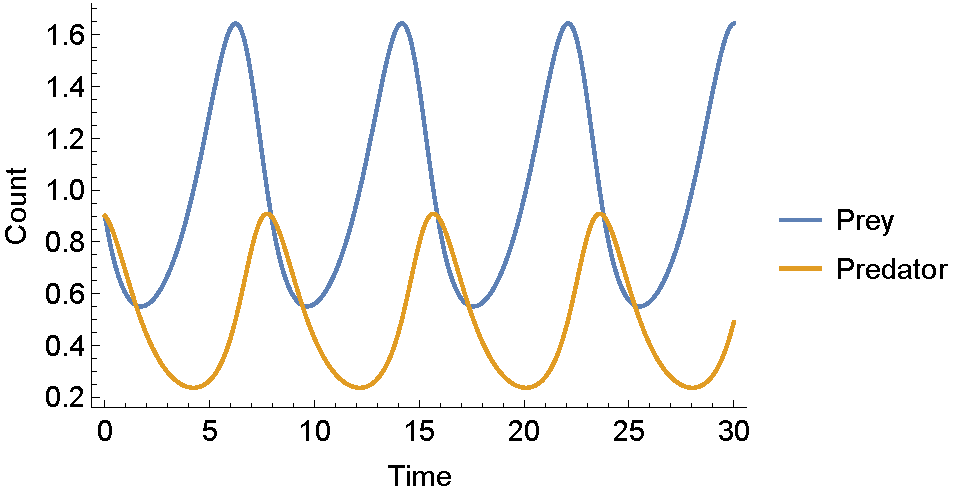
\includegraphics[width=1\textwidth]{./figures/lotka-volterra.pdf}}
	\end{figure}
		
\end{frame}


\begin{frame}
	\frametitle{Inference problem}
	
	\textbf{Problem:} Given prey series: $(x(0), x(10), x(20), x(30))$, 
	
	\vspace{0.2cm}
	
	can we infer $(\beta, \gamma)$?
	
	\vspace{0.5cm}
	
	\textbf{Answer:} try inference for simulated data! Here, we assume same set of parameters as before and
	
	\begin{equation}
	\tilde{x}(t) \stackrel{i.i.d.}{\sim} \text{normal}(x(t), 0.3),
	\end{equation}
	
	where $\tilde{x}(t)$ represents prey measurement at time $t$.
	
\end{frame}

\begin{frame}
	\frametitle{Measured prey series}
	
	With $\beta=4/3, \gamma=1$.
	
	\begin{figure}[ht]
		\centerline{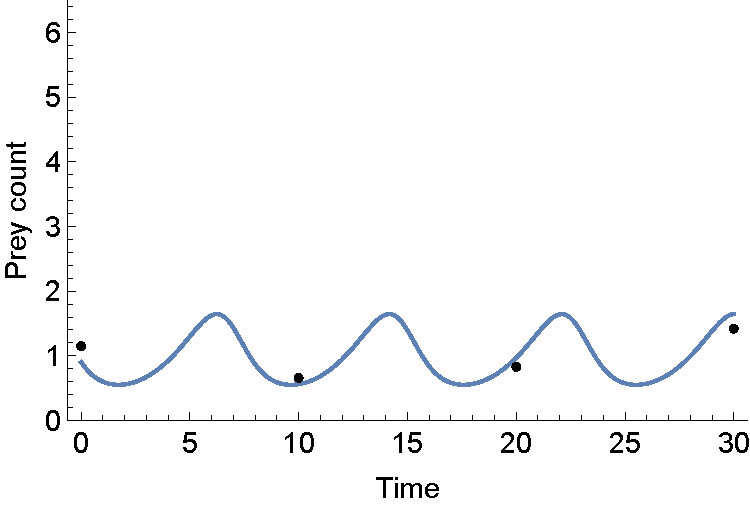
\includegraphics[width=1\textwidth]{./figures/lotka-volterra-infer-1.pdf}}
	\end{figure}
	
\end{frame}

\begin{frame}
	\frametitle{Other explanations}
	
	\begin{figure}[ht]
		\centerline{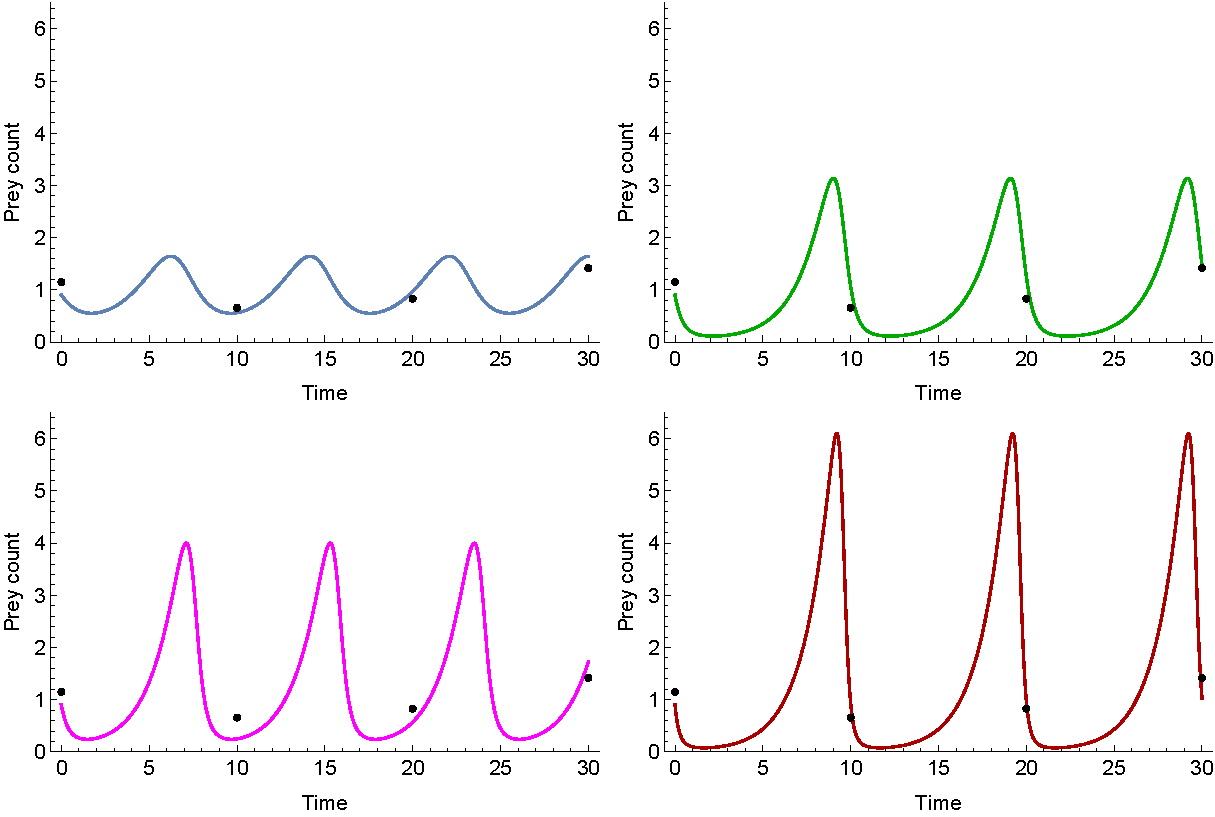
\includegraphics[width=1\textwidth]{./figures/lotka-volterra-inference-other.pdf}}
	\end{figure}
	
\end{frame}

\begin{frame}
	\frametitle{Inverse distance surface}
	
	\begin{figure}[ht]
		\centerline{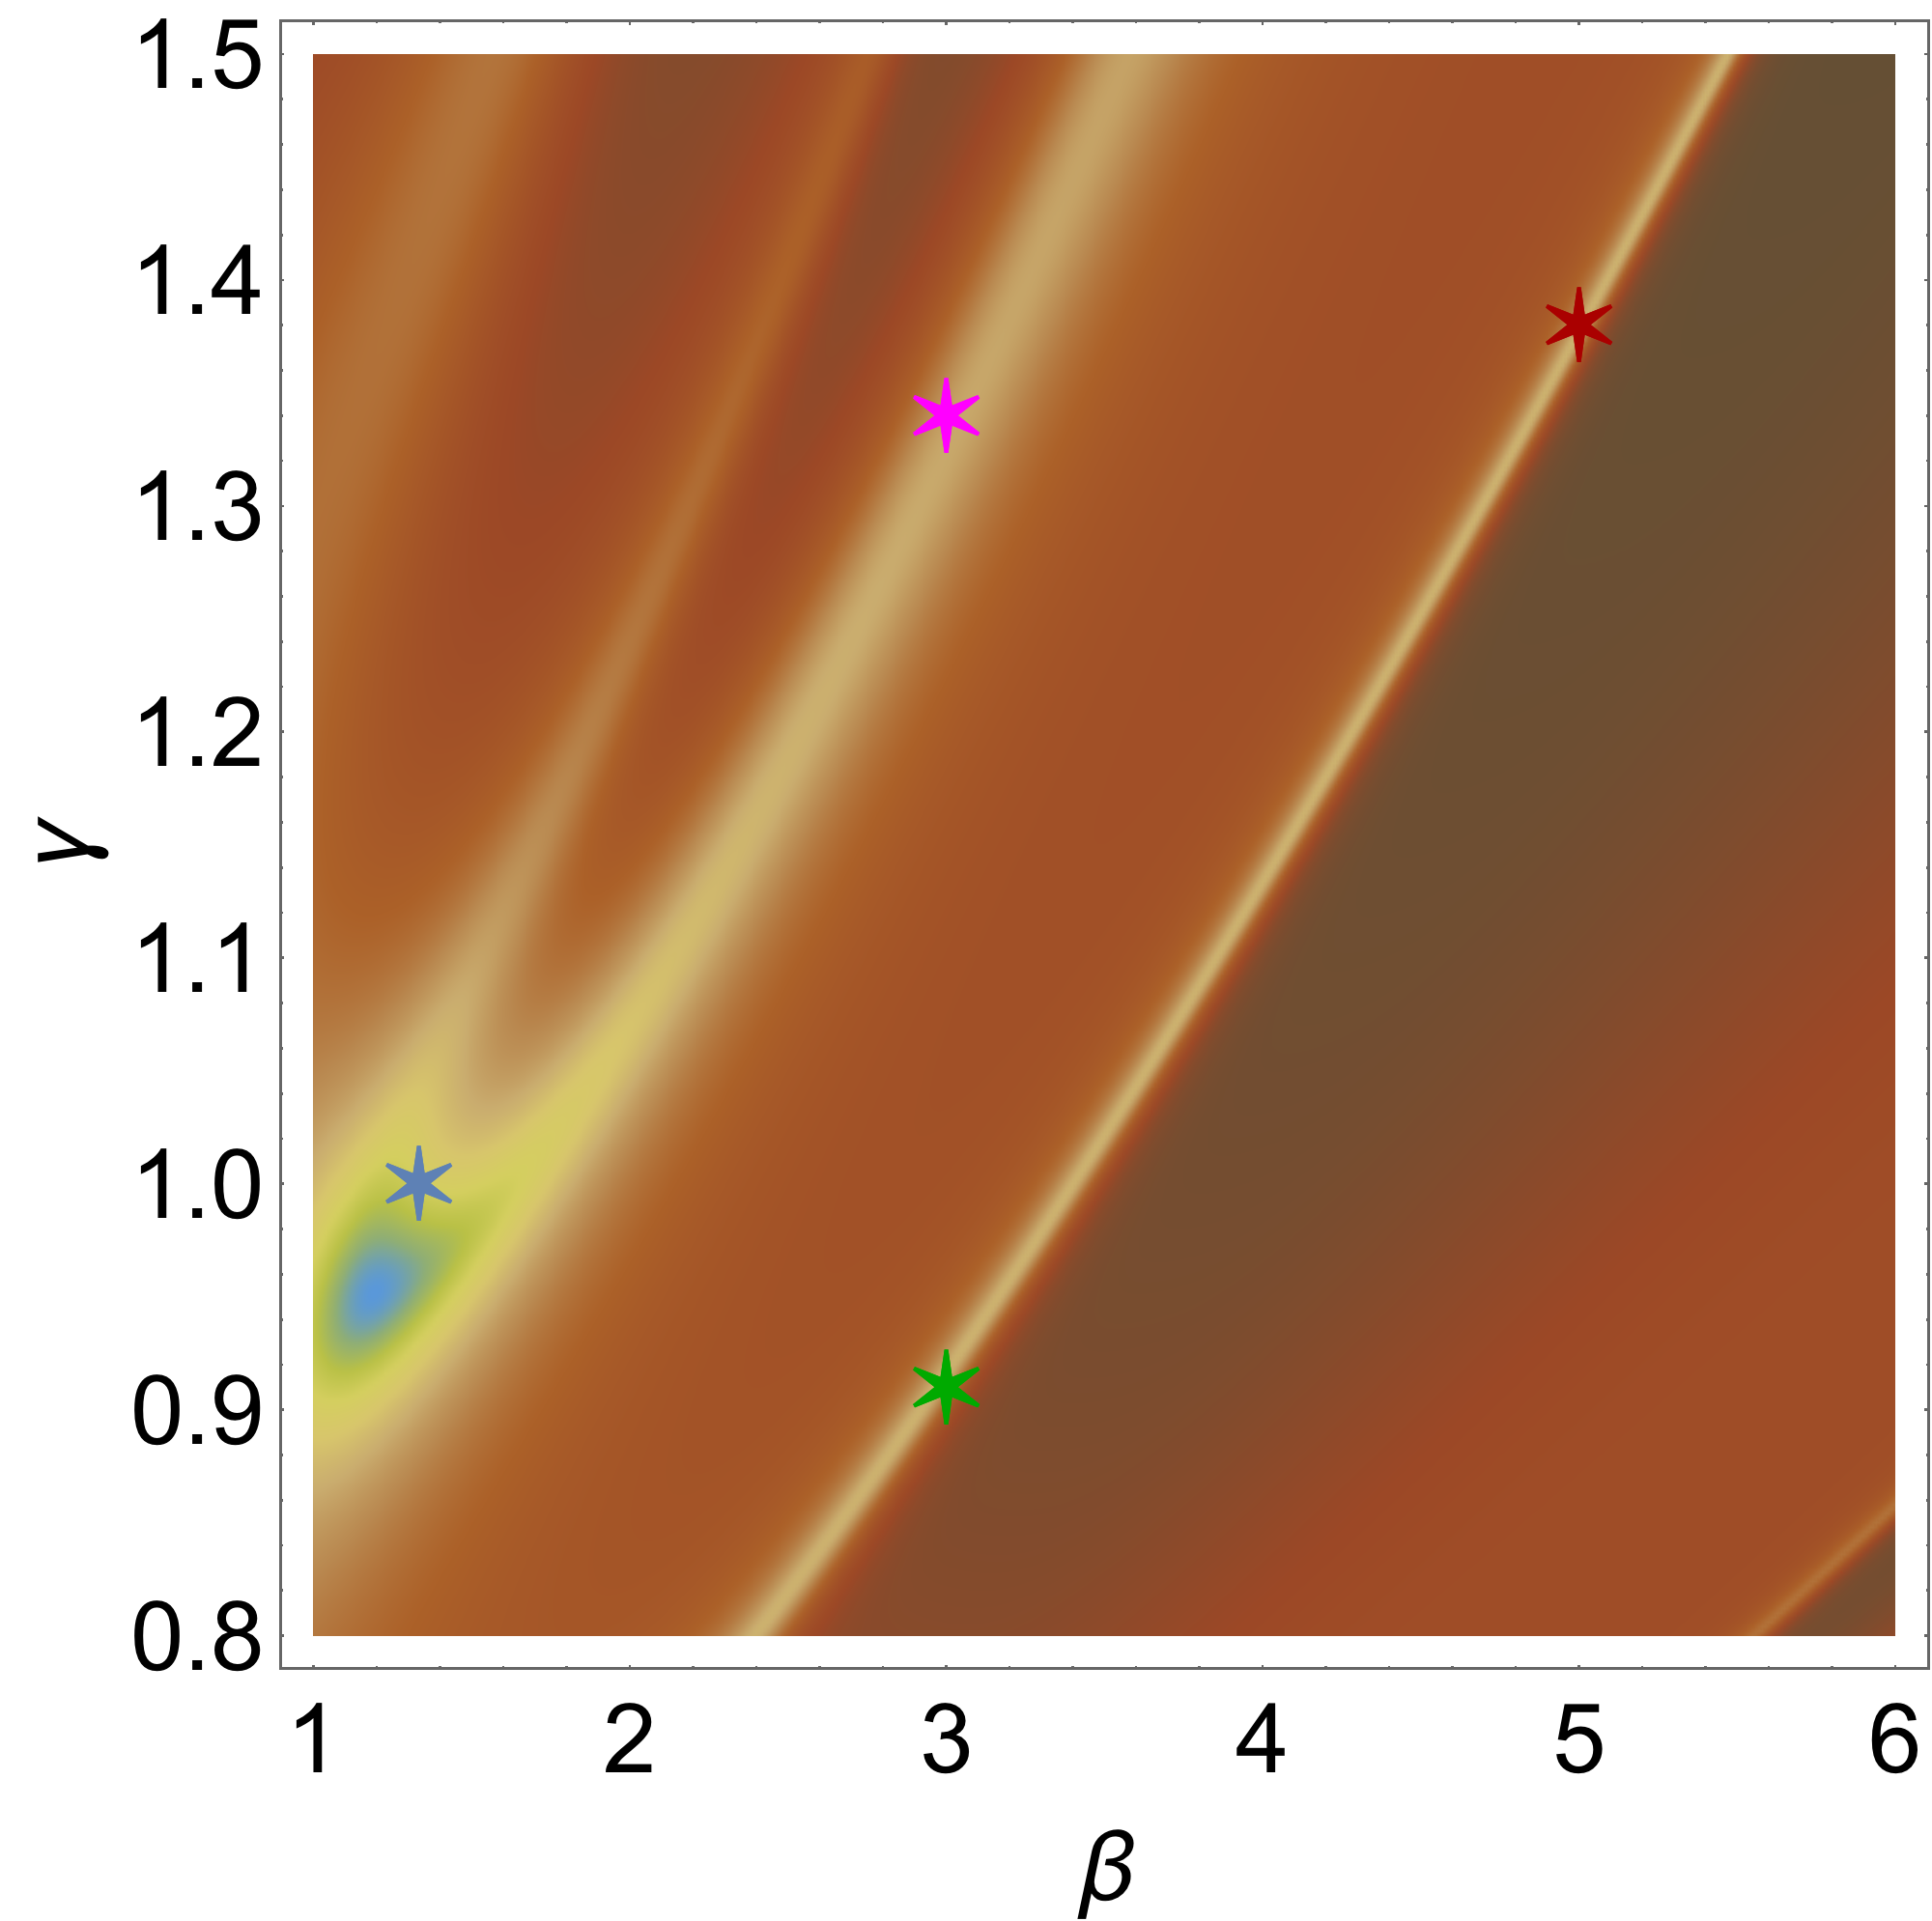
\includegraphics[width=0.7\textwidth]{./figures/lotka-volterra-inference-big.png}}
	\end{figure}
	
\end{frame}

\begin{frame}
	\frametitle{Lotka-Volterra inference problem: conclusions}
	
	\begin{equation}
	\text{sparse measurement} + \text{noise} \implies \sim \text{poorly identified}
	\end{equation}
	
	With the data to hand, it will be hard to estimate parameters with uncertainty. Solutions:
	
	\begin{itemize}
		\item Collect more data!
		\item Use pre-existing information to estimate parameters.
	\end{itemize}
	
\end{frame}

\begin{frame}
	\frametitle{Experimental design: the other side of the coin to inference}
	
	\begin{itemize}
		\item Experiments typically aim to estimate certain quantities
		\item If we have choice about how to measure a system, we can affect the sampling distribution of our estimators
		\item Simulated data can be used to decide how best to measure
	\end{itemize}
	
\end{frame}

\begin{frame}
	\frametitle{Using simulated data for experimental design}
	
	Repeat a number times at each experimental setup:
	\begin{enumerate}
		\item Simulate data using known parameters
		\item Run inference on parameters
		\item Compare true and estimated parameters
	\end{enumerate}
	
	\textbf{Note:} for useful experimental design, the simulated data should be as near to what you expect as possible!
\end{frame}

\begin{frame}
	\frametitle{Parameter sensitivities: another tool for experimental design}
	
	Suppose we have a model with solution:
	
	\begin{equation}
	y(t) = f(t, \theta),
	\end{equation}
	
	where $t$ is time and $\theta$ is a parameter we wish to estimate. Suppose this then gets used to calculate a log-likelihood for inference:
	
	\begin{equation}
	\mathcal{L} = \sum_{t=t_1}^{t_T} \log p(y(t)|f(t, \theta)).
	\end{equation}
	
\end{frame}

\begin{frame}
	\frametitle{Parameter sensitivities: another tool for experimental design}
	
	The precision of our estimates depends on how sensitive the log-likelihood is to choice of $\theta$. That is, on the magnitude of:
	
	\begin{equation}
	\frac{d\mathcal{L}}{d\theta}.
	\end{equation}
	
	This, in turn, depends on:
	
	\begin{equation}
	\frac{d f(t)}{d \theta}.
	\end{equation}
	
	So assessing the sensitivities of our model at various points in time to the parameters can also be used to guide experimental design.
	
\end{frame}

\begin{frame}
	\frametitle{That's it!}
	
	\Large Questions?
\end{frame}


\end{document}
